\chapter{Improved Style-based Tone Mapping}
\label{chp:b6}

Although style based tone mapping has achieved some success for consistently tone mapping different images, the image similarity method given in Section \ref{sec:operation} can be improved with the findings from the conducted user study. In this chapter, two modifications of this method that are made possible by the experimental findings of the user study is given. The first technique uses all of the image features utilized in Chapter~\ref{chp:b5} with different weights to estimate tone mapping parameters in the operation phase. Meanwhile, the second technique relates tone mapping parameters and image features for the estimation.

\section{Parameter Interpolation with All Features}
\label{sec:all_features}

In the first modification, the model features given in Table \ref{tab:table_feature} are extracted from the selected HDR image and calibration images. Then, the distances between these features are calculated separately using the corresponding distance metrics given in the same table. After that, the weighted average of these feature distances are calculated. The weights used are the coefficients of the logistic regression model (Equation \ref{eq:log_regression}) obtained from the user experiment, with the idea that less important features should also contribute less to the distance. This operation can be summarized with the following equation:

\begin{equation}
    d_i = \sum_{j=1}^{6}c_j d_j(\mathbf{f_i}, \mathbf{f_{ij}})
\end{equation}

where $c_j$ is the coefficient of the $j^{th}$ feature, $\mathbf{f_j}$ is the $j^{th}$ feature of the input image, $\mathbf{f_{ij}}$ is the same for the $i^{th}$ calibration image, and finally $d_j$ is the distance metric for the $j^{th}$ feature. The result $d_i$ represents the combined distance between the input image and the corresponding calibration image. These combined distances are calculated between the selected HDR image and all calibration images. The tone mapping parameters for the selected HDR image are then interpolated using inverse distance transform as in Equation \ref{eq:inv_distance_transform}. This method differs from the initially presented approach in several aspects: 

\begin{itemize}
    \item Using a different and more representative set of features, luminance which is one of the most important features of HDR images has a separate feature vector,
    \item More suitable distance metrics for feature types, for example, EMD takes into account bin proximity for calculating differences between histograms,
    \item Instead of using a single fused feature vector, each feature distance calculated separately,
    \item Employing a weighted average of feature vector distances with weights obtained from a user experiment, compared to using equal weight.
\end{itemize}

In Figure~\ref{fig:algo_updated}, the modified style-based tone mapping algorithm is shown. Note that while the calibration phase has not changed, the operation phase has been adjusted with the changes listed above compared to the initial version of the algorithm given in Figure~\ref{fig:calibration_operation}. 

\begin{figure}
    \centering
    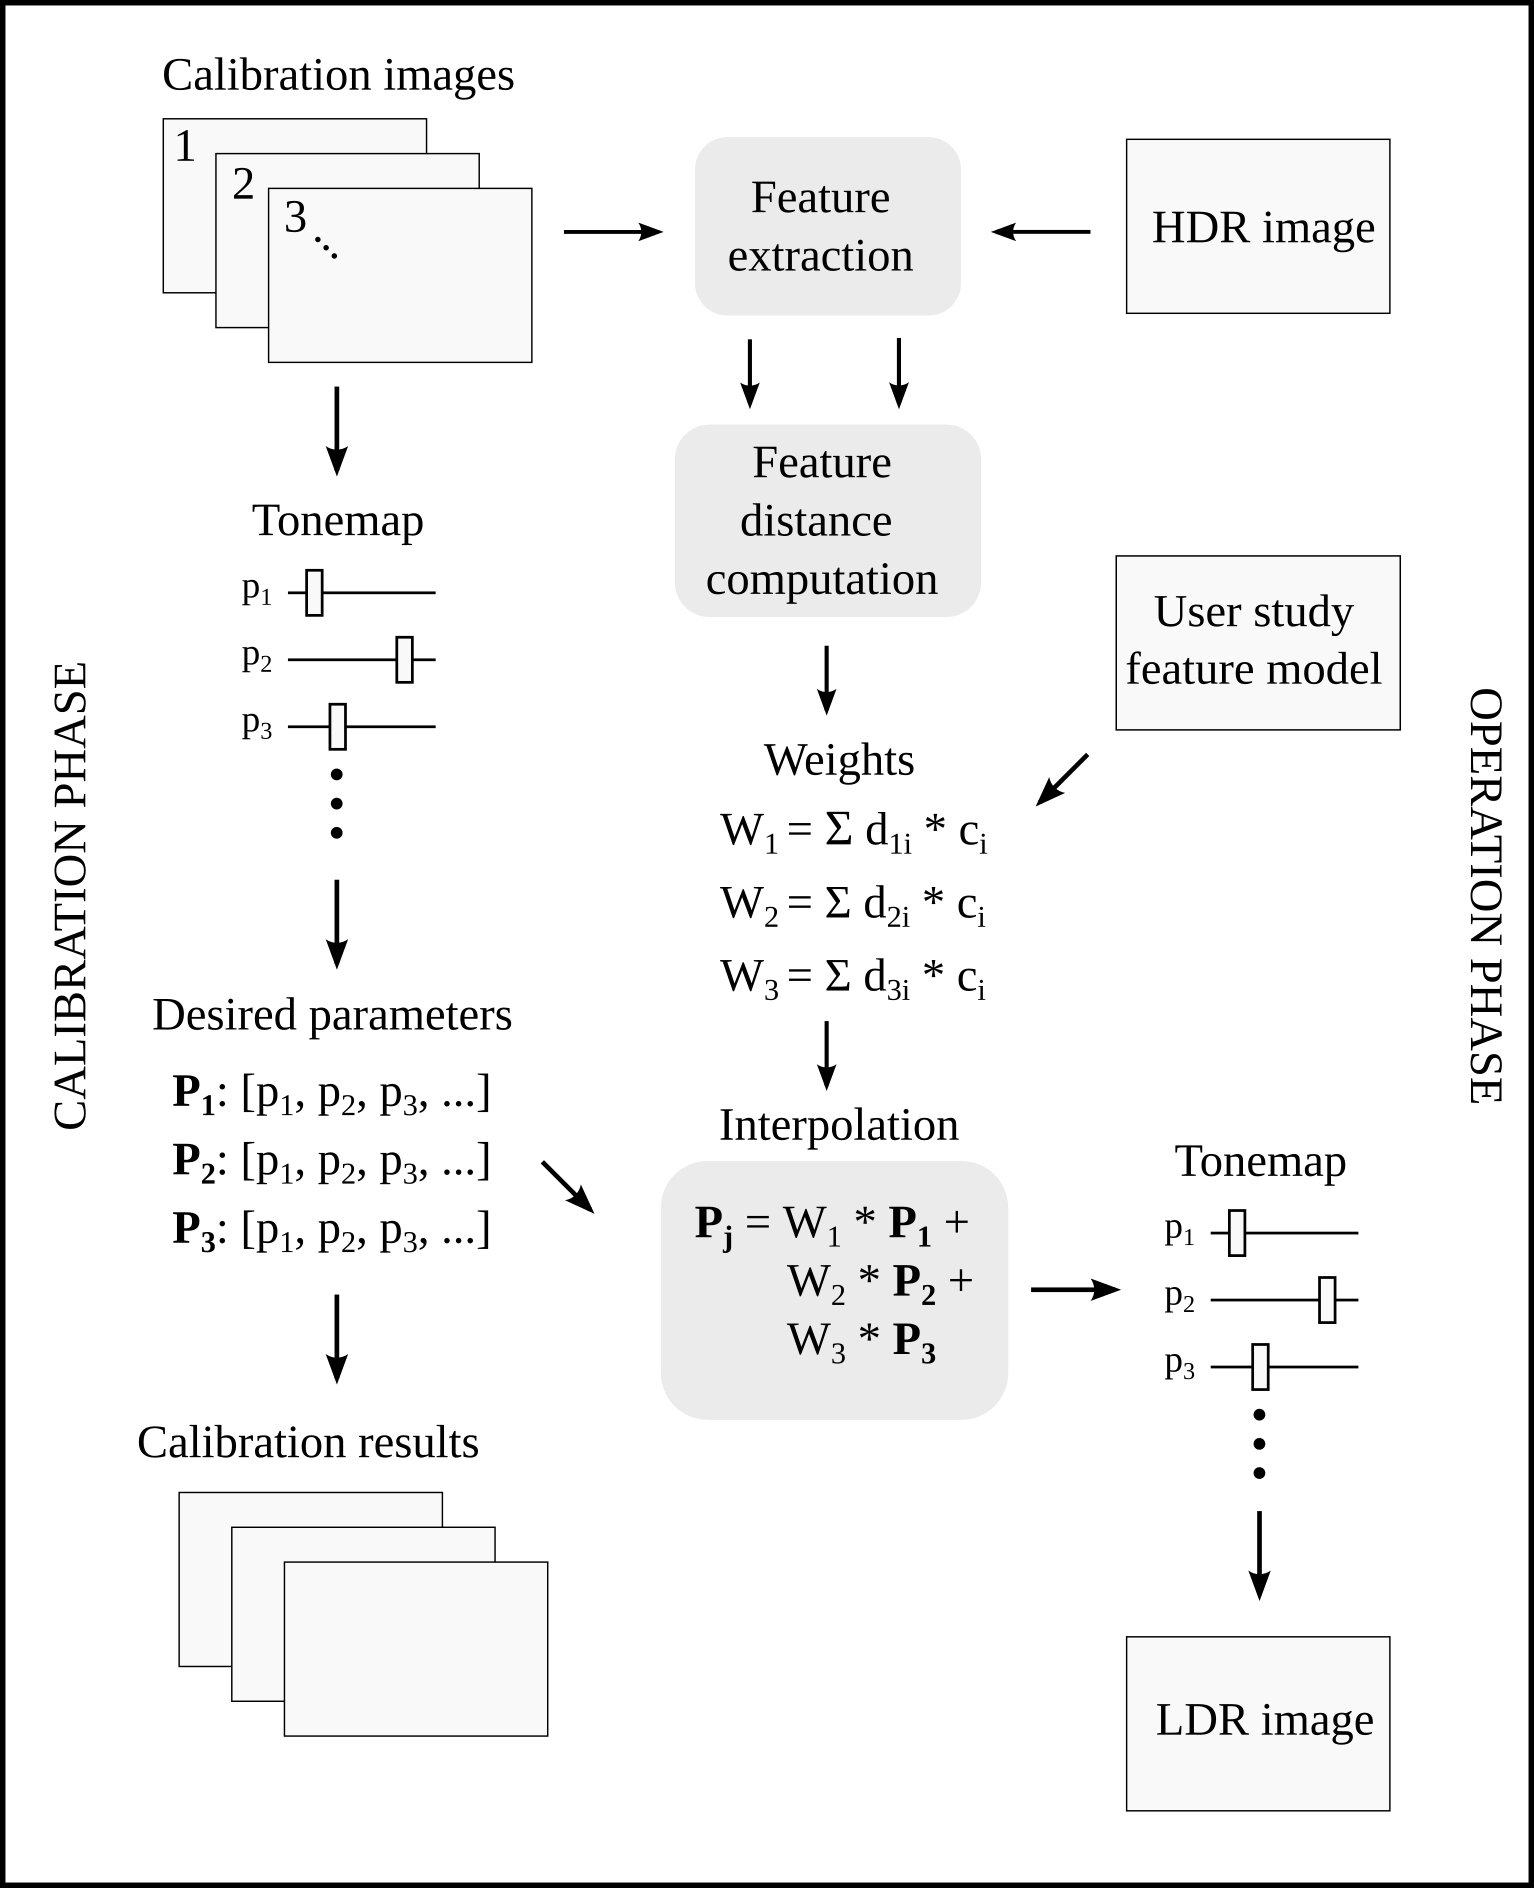
\includegraphics[width=\textwidth]{figures/algorithm_updated.png}
    \caption{Modified style-based tone mapping algorithm with the findings of the user experiment. Compared to the initial method given in Figure~\ref{fig:calibration_operation}, more representative set of features are extracted and distances between these features are computed separately. Besides, instead of using equal weights on feature distances, the weights estimated from user study are employed.}
    \label{fig:algo_updated}
\end{figure}

\section{Parameter Interpolation with Related Features}
\label{sec:related_features}
While the previous approach calculates a single distance value between the given image and calibration images and use this value to interpolate all tone mapping parameters, the second modification described in this section relates the model features with the tone mapping parameters and interpolates individual tone mapping parameters with different weights. In order to achieve this, the relationships defined in Table~\ref{tab:feature_mapping} are used.

\begin{table}
\caption{Model features used for interpolation of tone mapping parameters.}
\centering
\begin{tabular}{l | l}
\label{tab:feature_mapping}
\textbf{Tone mapping parameter} & \textbf{Model feature}\\
\hline
Brightness ($t_b$) & Luminance \\
Contrast ($t_c$) & Luminance \\
Black point ($t_{bp}$) & Luminance \\
White point ($t_{wp}$) & Luminance \\
Color saturation ($t_s$) & Color \\
Small detail strength ($t_{\lambda_s}$) & Texture \\
Medium detail strength ($t_{\lambda_m}$ ) & Texture \\
Large detail strength ($t_{\lambda_l}$) & Texture
\end{tabular}
\end{table}


As an example, the brightness parameter $t_b$ is computed by interpolating the $t_{b_i}$ parameters of the calibration images by using the similarity between the luminance features:

\begin{equation}
   t_b = { {\sum_{i=1}^N { {1} \over {d_{lum} (lum, lum_i)} } t_{b_i} } \over {\sum_{i=1}^N} { {1} \over {d_{lum} (lum, lum_i)} } }
\end{equation}

Other tone mapping parameters that are related to the model features are interpolated analogously. Because GIST and deep learning features are not directly linked to a specific appearance phenomenon but are measures of overall similarity between the given images, they are not directly linked to specific tone mapping parameters. Instead these features are experimented with merging them using the individually interpolated parameters as follows: 

\begin{equation}
   \mathbf{t} = w_0\mathbf{t_0} + w_1\mathbf{t_1} + w_2\mathbf{t_2}, 
\end{equation}

where $\mathbf{t_0}$ represents individually interpolated TMO parameters (given in Table~\ref{tab:feature_mapping}), $\mathbf{t_1}$ TMO parameters interpolated as a whole using GIST similarity only, and $\mathbf{t_2}$ TMO parameters interpolated as a whole using solely deep learning feature similarity. The weights control the influence of TMO parameters that are computed by using these different approaches.

\section{Results}
In Figure~\ref{FigStyle}, several results are compared that obtained by using the initial style based tone mapping method as well as with the two modifications proposed in the previous sections, Section~\ref{sec:related_features} and Section~\ref{sec:all_features}. 

In the first row of the figure, the tone mapping results of the ``Paul Bunyan'' scene from the HDR Photographic Survey~\cite{fairchild2007hdr} is shown. This scene depicts a bright outdoors environment with colorful foreground objects. It may be noted that all results are similar but the individual parameter interpolation with equally weighted GIST and deep learning features (d) has slightly higher contrast (please refer to Appendix~\ref{app:results} with high resolution images for better comparison). The overall \emph{candy} style is preserved in all images. 

In the second row of the figure, ``Peppermill'' night scene from the same dataset is shown. This is a night scene of a street with some bright lights and banners. For this scene the difference of the second modification, parameter interpolation with related features, is more clear as images in (c) and (d) exhibit a darker rendering, which is more suitable for a night scene. The reason for this darkening effect is that the brightness parameter, $t_b$, for tone mapping becomes more similar to the $t_b$ parameter of the night image in the calibration images due to the similarity of the \emph{luminance} features between these images. The addition of GIST and deep learning features with equal weight in (d) yields a slightly brighter image compared to (c). Similar to the results of the previous image overall \emph{candy} style is preserved also in this image. Appendix~\ref{app:results} has higher resolution versions of the results for more clear observation of the differences.


\afterpage{
\begin{landscape}
\begin{figure}
\begin{subfigure}[b]{0.40\textwidth}
    \centering
    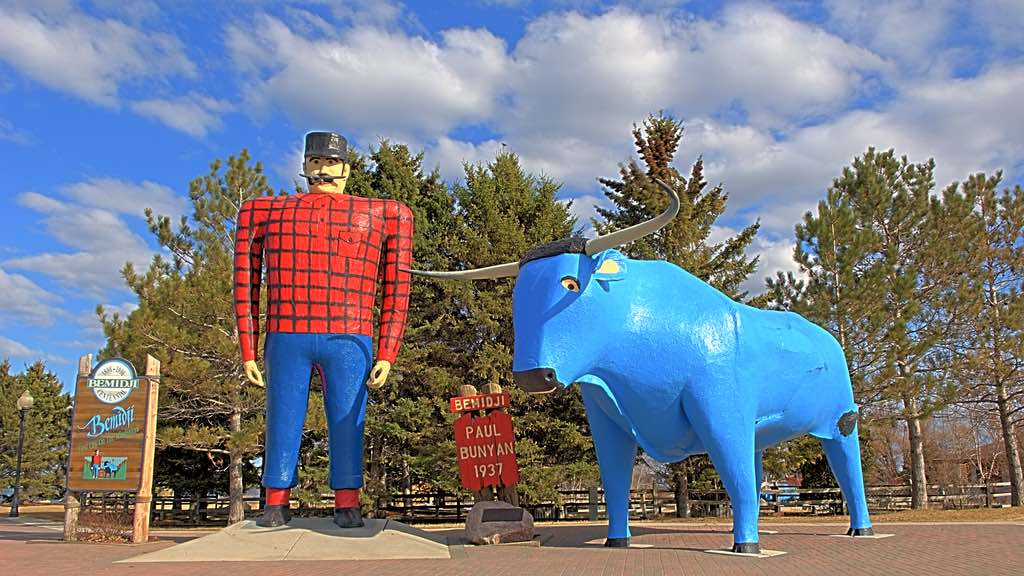
\includegraphics[width=\textwidth]{figures/chapter5/style_based/PaulBunyan_hdrcandy_v1_small.jpg}
    \caption{Initial}
    \label{FigStyle:original_paul_bunyan}
\end{subfigure}\hfill
\begin{subfigure}[b]{0.40\textwidth}
    \centering
    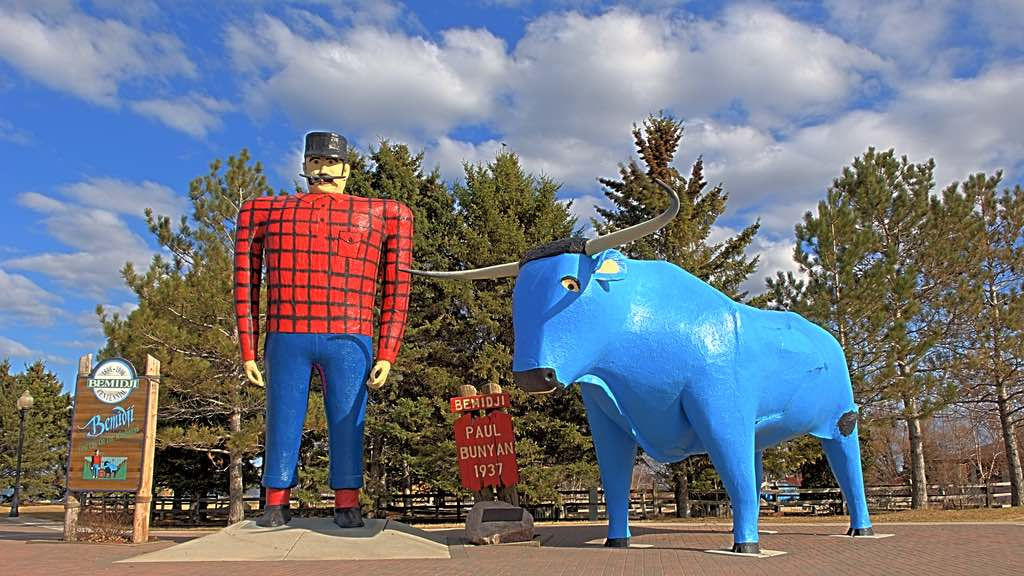
\includegraphics[width=\textwidth]{figures/chapter5/style_based/PaulBunyan_hdrcandy_v2_small.jpg}
    \caption{Version I}
    \label{FigStyle:VerI_paul_bunyan}
\end{subfigure}\hfill
\begin{subfigure}[b]{0.40\textwidth}
    \centering
    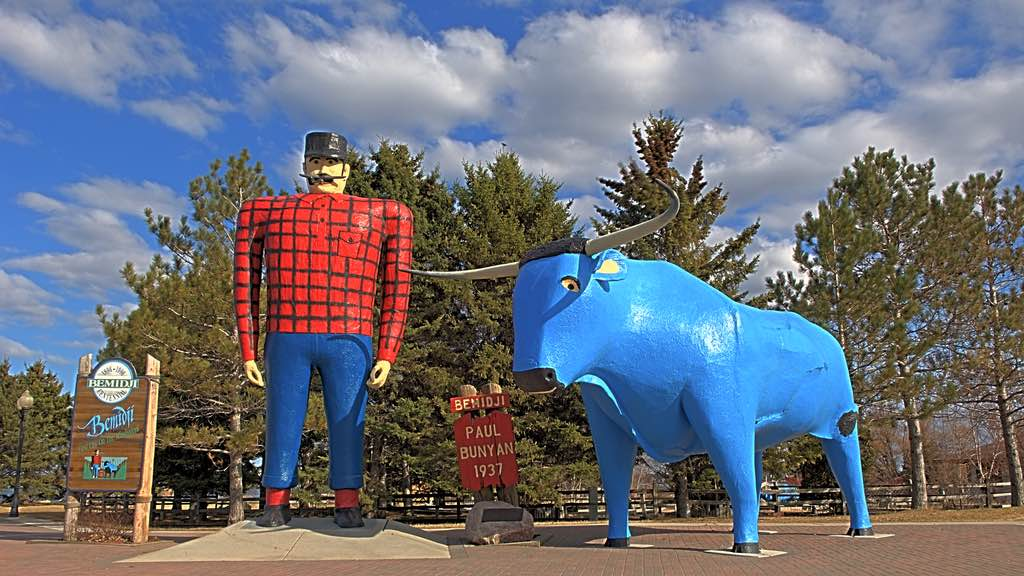
\includegraphics[width=\textwidth]{figures/chapter5/style_based/PaulBunyan_hdrcandy_w0_1_small.jpg}
    \caption{$w_0 = 1$, $w_1 = w_2 = 0$}
    \label{FigStyle:VerIIa_paul_bunyan}
\end{subfigure}\hfill
\begin{subfigure}[b]{0.40\textwidth}
   \centering
    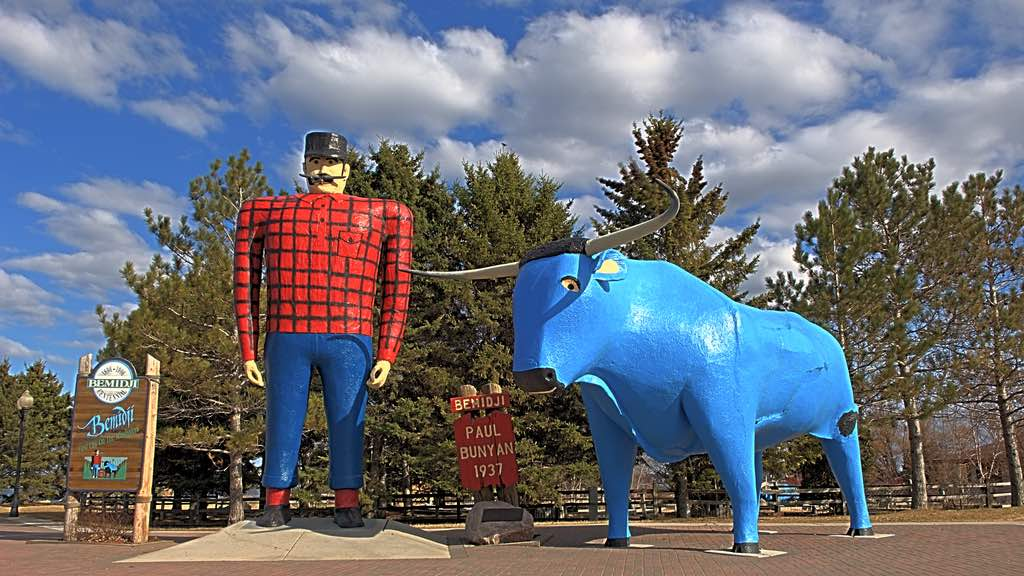
\includegraphics[width=\textwidth]{figures/chapter5/style_based/PaulBunyan_hdrcandy_w0_w1_w2_small.jpg}
    \caption{$w_0 = w_1 = w_2 = \frac{1}{3}$}
    \label{FigStyle:VerIIb_paul_bunyan}
\end{subfigure}\\
\begin{subfigure}[b]{0.40\textwidth}
    \centering
    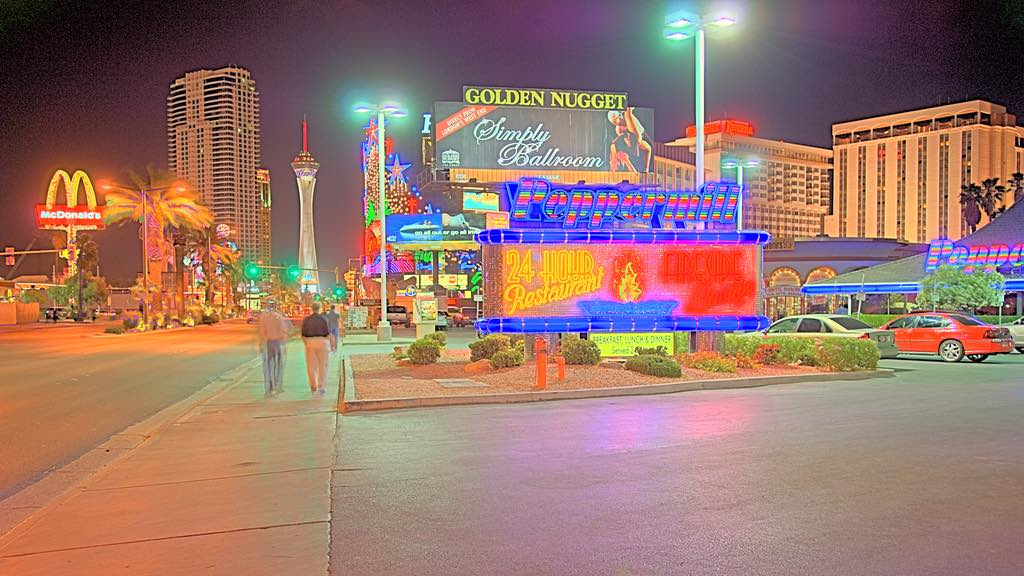
\includegraphics[width=\textwidth]{figures/chapter5/style_based/Peppermill_hdrcandy_v1_small.jpg}
    \caption{Initial}
    \label{FigStyle:original_peppermill}
\end{subfigure}\hfill
\begin{subfigure}[b]{0.40\textwidth}
    \centering
    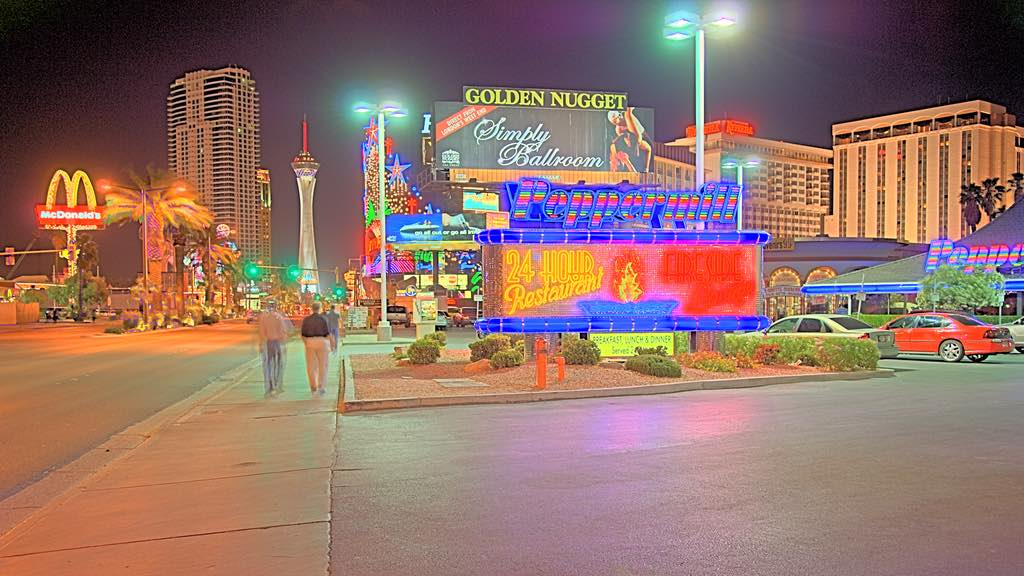
\includegraphics[width=\textwidth]{figures/chapter5/style_based/Peppermill_hdrcandy_v2_small.jpg}
    \caption{Version I}
    \label{FigStyle:VerI_peppermill}
\end{subfigure}\hfill
\begin{subfigure}[b]{0.40\textwidth}
    \centering
    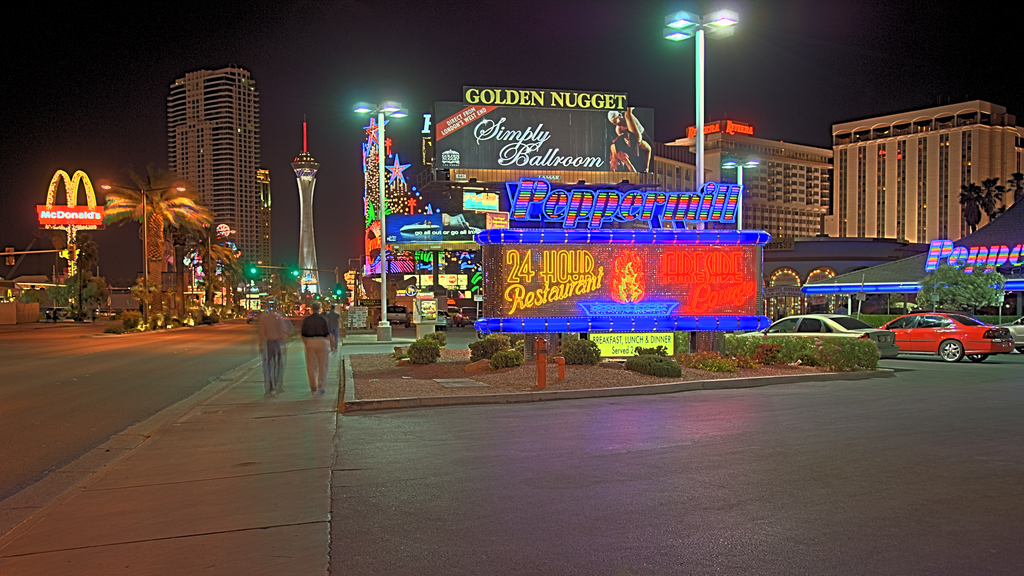
\includegraphics[width=\textwidth]{figures/chapter5/style_based/Peppermill_hdrcandy_w0_1.png}
    \caption{$w_0 = 1$, $w_1 = w_2 = 0$}
   \label{FigStyle:VerIIa_peppermill}
\end{subfigure}\hfill
\begin{subfigure}[b]{0.40\textwidth}
    \centering
    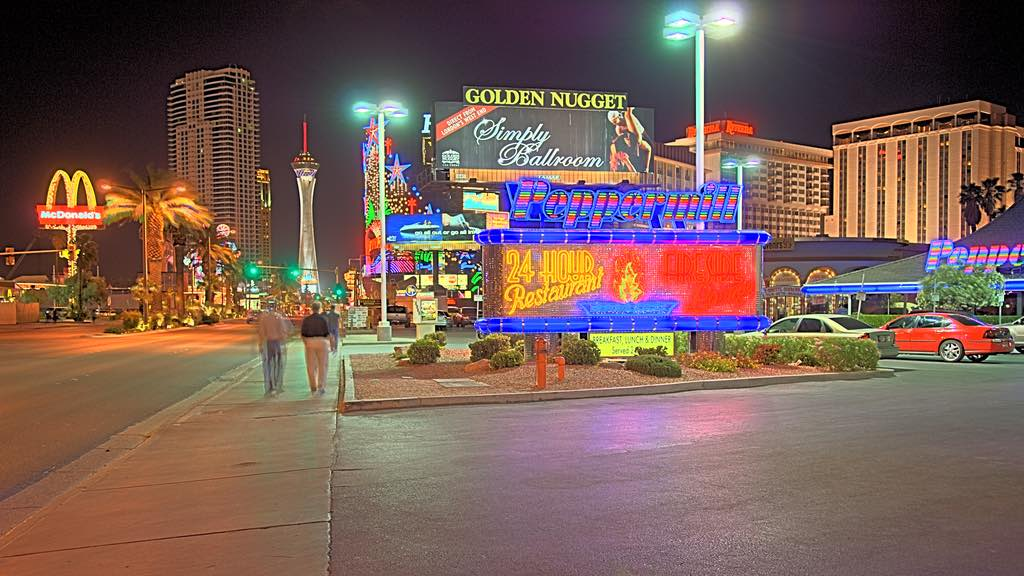
\includegraphics[width=\textwidth]{figures/chapter5/style_based/Peppermill_hdrcandy_w0_w1_w2_small.jpg}
    \caption{$w_0 = w_1 = w_2 = \frac{1}{3}$}
    \label{FigStyle:VerIIb_peppermill}
\end{subfigure}\hfill
\caption{Application of the user study findings for the style-based tone mapping
    problem.  Initial results are shown in the first column, followed
        by Version I in the second column and two variants of Version II
in the last two columns.}
\label{FigStyle}
\end{figure}
\end{landscape}}
